\def\OtherAuthors{, Magnus~Dunn, Kaden~Bernhard, Elisabeth~Belanger, Eric~Jia}
\SetTitle{31}{Quantum Fourier Transform}{Inverse of Phase Estimation}{31}

\begin{frame}{Overview}{What will we study?}

\begin{itemize}
    \item The \href{https://en.wikipedia.org/wiki/Fourier_transform}{Fourier Transform} is well known in physics and mathematics for its ability to represent a time-based signal as a summation of frequencies that approximates or yields the original signal.
    \item We will review the basics of the classical Fourier transform.
    \item We will study the Quantum Fourier Transform (QFT), but it turns out that this circuit is simply the \href{https://en.wikipedia.org/wiki/Quantum_phase_estimation_algorithm}{Phase Estimation} circuit, executed in reverse.
    \item The QFT is at the center of important quantum algorithms, such as \href{https://en.wikipedia.org/wiki/Shor\%27s_algorithm}{Shor's Algorithm}, which we study next.
\end{itemize}
\end{frame}

\section*{Classic Fourier}

\begin{frame}{Classic Fourier}{Overview}
\Vskip{-3em}\TwoColumns{%
\Vskip{-2.5em}\begin{center}
        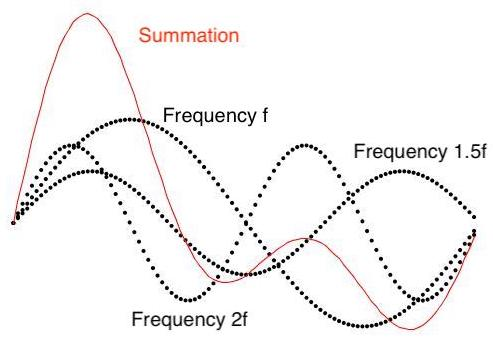
\includegraphics[width=0.8\textwidth]{310/instr.jpeg}
    \end{center}
}{%
\only<1>{%
\begin{itemize}
    \item Sine waves are plotted above at frequencies $f$, $2f$, and $1.5f$.
    \item If those frequencies sound at the same time, the red wave shows the resulting signal that reaches our ears:  the summation of the three black waves.
\end{itemize}
}%
\only<2>{%
Fourier analysis expresses the red wave in terms of the black waves, whose summation equals or approximates the red wave.  In this example, each black wave has the same weight.  In the more general setting, Fourier analysis determines the weight of each sine wave that contributes to the red wave.
}%
}%
%
\Vskip{-1.5em}\begin{itemize}
    \item Remarkably, our brain performs Fourier analysis on the red signal, informing us that we hear a pitch, an octave above that pitch, and the ``fifth'' in between the other two pitches.
    \item This is how our brain can distinguish the sounds of trombones, clarinets, violins, and pipe organs.
   
\end{itemize}%

\end{frame}

\begin{frame}{Watch these videos about the Fourier transform}{From Grant Sanderson's \href{https://www.3blue1brown.com/}{3blue1brown}}

\begin{description}
    \item[\href{https://www.youtube.com/watch?v=spUNpyF58BY}{Visual introduction to Fourier}]  Given a time-series signal, how do we create its correspondency graph of frequency intensities?
    \item[\href{https://www.youtube.com/watch?v=r6sGWTCMz2k}{How Fourier works}]  How do we use the frequencies and their intensities to create a time-series signal?
    \item[\href{https://www.youtube.com/watch?v=MBnnXbOM5S4}{Uncertainty principle, regarding Fourier transforms}]  further enrichment
\end{description}
    
\end{frame}


\begin{frame}{Quantum Fourier}{As compared with Phase Estimation}
\TwoColumns{%
Phase estimation considers the state
\[
\QState{} = \RootTwoN{n}\SumPH{y}{n} \ExpPhase{2\pi \frac{x}{2^n} y} \ket{y}
\]
and computes \ket{x}.
}{%
Quantum Fourier takes a basis state \ket{x} and generates the state
\begin{align*}
\QState{} &= \RootTwoN{n}\SumPH{y}{n} \ExpPhase{2\pi \frac{x}{2^n} y} \ket{y} \\
   &= \RootTwoN{n}\SumPH{y}{n} \ExpPhase{2\pi \frac{y}{2^n} x} \ket{y} 
\end{align*}
}%
\BigSkip{}
So, one operation is the reverse of the other.  We will see this clearly when discussing the circuit for QFT.
\end{frame}


{%
\def\QT#1#2{\ExpPhase{2\pi \alert<#2>{\frac{#1}{2^n} x}} \ket{#1}}
\def\QTO#1#2{\visible<#2->{\ExpPhase{\frac{2\pi}{2^n}\, \alert<#2>{#1\cdot x}}\ket{#1}}}
\def\Space{\hbox to 4em{\hss}}
\begin{frame}{The summation in QFT}{Viewed two different ways}
\Vskip{-3.2em}\[ \QFT(\ket{x}) = \RootTwoN{n}\SumPH{y}{n} \ExpPhase{2\pi \frac{y}{2^n} x} \ket{y}\]
\Vskip{-2em}\TwoColumns{%
Fractions of $x$ around the unit circle:
\begin{align*}
       &= \RootTwoN{n}   \left[\  \QT{0}{2} \right. \\
         &\Space{}+ \QT{1}{3} \\
         &\Space{}+ \QT{2}{4} \\
         &\Space{}+ \RVDots{} \\
         &\Space{}+ \left. \QT{2^{n-1}}{5} \ \right] 
\end{align*}
}{%
Multiples of $x$:
\begin{align*}
       &= \RootTwoN{n}   \left[\  \QTO{0}{2} \right. \\
         &\Space{}+ \QTO{1}{3} \\
         &\Space{}+ \QTO{2}{4} \\
         &\Space{}+ \RVDots{} \\
         &\Space{}+ \left. \QTO{2^{n-1}}{5} \ \right] 
\end{align*}
}%
\BigSkip{}
The $\cdot$ is simple multiplication, and $x$ takes on a value in $[0,1, \ldots, 2^{n}-1]$.
\end{frame}}

{
\def\QZ#1{\ExpPhase{\frac{2\pi}{2^n}\,#1\cdot 0}\,\ket{#1}}
\def\Space{\hbox to 4em{\hss}}
\begin{frame}{Some observations}{\QFT(\ket{0}) is familiar}
\TwoUnequalColumns{0.6\textwidth}{0.4\textwidth}{%
\begin{align*}
      \QFT(\ket{0}) &= \RootTwoN{n}   \left[\  \QZ{0} \right. \\
         &\Space{}+ \QZ{1} \\
         &\Space{}+ \QZ{2} \\
         &\Space{}+ \RVDots{} \\
         &\Space{}+ \left. \QZ{2^{n-1}} \ \right] 
\end{align*}
}{%
\visible<2->{%
\begin{align*}
&= \RootTwoN{n}   \left[\ \ \  \ket{0} \right. \\
         &\Space{}+ \ket{1} \\
         &\Space{}+ \ket{2} \\
         &\Space{}+ \RVDots{} \\
         &\Space{}+ \left. \ket{2^{n-1}} \ \right]\\
         &= \Hadamard(\ket{0})
\end{align*}
}%
}
    
\end{frame}
}

{
\def\HD#1{\NegOneExp{\DotP{x}{#1}}\,\ket{\,#1\,}}
\def\QZ#1{\ExpPhase{\frac{2\pi}{2^n}}}
\def\Space{\hbox to 3.5em{\hss}}
\begin{frame}{\QFT{} and \Hadamard{}}{Treatment of a basis state}
While \QFT{} and \Hadamard{} provide the same result on basis state \QZero{}, they treat other states differently:
\BigSkip{}
\TwoColumns{%
\only<1>{%
The \Hadamard{} operator places a plus or minus sign on each basis vector \ket{y}:
\[ \NegOneExp{\DotP{x}{y}}\ \ket{y} \]
where \DotP{x}{y} is computed as $\oplus\left(\And{x}{y}\right)$: the xor-reduction of the
bit-wise ``and'' of $x$ and $y$.
\MedSkip{}            
Thus, each basis state \ket{x} induces a specific pattern of $\pm 1$ on the superposition created by the \Hadamard{} operator.
}%
\only<2>{%
\begin{align*}
      \QFT(\ket{0}) &= \RootTwoN{n}   \left[\  \QZ{0} \right. \\
         &\Space{}+ \QZ{1} \\
         &\Space{}+ \QZ{2} \\
         &\Space{}+ \RVDots{} \\
         &\Space{}+ \left. \QZ{2^{n-1}} \ \right] 
\end{align*}
}%
}{%
\only<1,3>{%
\Vskip{-3em}\begin{align*}
\Hadamard\left(\ket{x}\right) &= \RootTwoN{n}   \left[\ \ \  \HD{0} \right. \\
         &\Space{}+ \HD{1} \\
         &\Space{}+ \HD{2} \\
         &\Space{}+ \RVDots{} \\
         &\Space{}+ \left. \HD{2^{n-1}} \ \right]
\end{align*}}%
\only<2>{%
}%
}
    
\end{frame}


\subsection*{Ron}
\begin{frame}{Fourier transform}{As a unitary matrix}
    
\end{frame}

\begin{frame}{The Fourier matrix is unitary}{Sketch of proofs on next slides}

If $U$ is a quantum Fourier transform matrix, then
\begin{itemize}
  \item The columns of $U$ are \href{https://en.wikipedia.org/wiki/Orthogonality}{orthogonal}
  \item The columns of $U$ have \href{https://en.wikipedia.org/wiki/Unit_vector}{unit length}
  \item $U\times \Conj{U}=\Conj{U}\times U = \Identity$
\end{itemize}
    
\end{frame}

\subsection{Ron}
\begin{frame}{The columns are orthogonal}{Proof}
    
\end{frame}

\subsection*{Elisabeth and Eric}
\begin{frame}{The columns have unit length}{Proof}
\only<1-4>{
\begin{itemize}
    \item Let n = Number of Qubits
    \item Let N = $2^{n}$ (Number of Quantum States)
    \item Let w = \ExpPhase{\frac{2\pi}{N}}
\end{itemize}
\TwoColumns{%
\visible<2-4>{
A column $C_y$ of the QFT matrix is: \\
\[
|C_y\rangle=\frac{1}{\sqrt{N}}\begin{bmatrix}
   1 \\
   {w^{1\cdot y}}\\
   {w^{2\cdot y}}\\
   . \\
   . \\
   . \\
   {w^{(N-1)\cdot y}}\\
\end{bmatrix}
\]
}
}{
\visible<3,4>{
The columns of a QFT matrix have unit length such that $\sqrt{\langle C_y | C_y \rangle}$ = 1 where \\
$\langle C_y |$ is the conjugate transpose of $|C_y\rangle$
}
\visible<4>{
\[
\langle C_y |=\frac{1}{\sqrt{N}}
\begin{bmatrix}
    1 & \overline{{w^{1\cdot y}}} & ... & \overline{{w^{(N-1)\cdot y}}} 
\end{bmatrix}
\]
}
}
}
\begin{Reasoning}
\Reason{5}{First we take the inner product of the column y and its conjugate transpose.}
\Reason{6}{First we take the inner product of the column y and its conjugate transpose.}
\Reason{7}{Since $w$ is exponential, we take the conjugate by negating its exponential}
\Reason{8}{This product can be written as a summation over k.}
\Reason{9}{We can replace $w$ by $e^{\frac{-2\pi i}{N}k}$.}
\Reason{10}{The exponentials add to 0, leaving a summation over just a constant.}
\Reason{11}{Taking the square root of both sides, we get a length equal to 1.}
\end{Reasoning}
\ScrollProof{5}{6}{%
\begin{align}
\Next{\Two}{
        \langle C_y | C_y \rangle=\frac{1}{\sqrt{N}}
        \begin{bmatrix}
            1 & \overline{{w^{1\cdot y}}} & ... & \overline{{w^{(N-1)\cdot y}}} 
        \end{bmatrix}
        \frac{1}{\sqrt{N}}
        \begin{bmatrix}
           1 \\
           {w^{1\cdot y}}\\
           {w^{2\cdot y}}\\
           . \\
           . \\
           . \\
           {w^{(N-1)\cdot y}} \\
        \end{bmatrix}
      }
\Last{&  \\ =  \frac{1}{N}(1+
        \overline{{w^{1\cdot y}}}{w^{1\cdot y}}+...+
        \overline{{w^{(N-1)\cdot y}}}{w^{(N-1)\cdot y}}) 
        \\}
        \end{align}
}%
\ScrollProof{7}{9}{%
\begin{align}
\Next{\Three}{ \\ \langle C_y | C_y \rangle = \frac{1}{N}(1+
        w^{-y}w^{y}+...+
        w^{(N-1)(-y)}w^{(N-1)(y)}) 
        \\ }
\Next{\Two}{ 
        \\ =\frac{1}{N}
        \SumPH{k}{n} {w^{-yk}}{w^{yk}} \\}
\Last{ & \\ =\frac{1}{N}
        \SumPH{k}{n} {e^{\frac{-2\pi i}{N}k}} {e^{\frac{2\pi i}{N}k}}\\ }
\end{align}
}
\ScrollProof{10}{11}{%
\begin{align}
\Next{\Two}{\\  \langle C_y | C_y \rangle=\frac{1}{N}
        \SumPH{k}{n} {e^{0}}=\frac{1}{N}({2^{n}-1})=\frac{1}{N}\cdot N=1 \\}
\Last{\sqrt{\langle C_y | C_y \rangle } = \sqrt{1} = 1 }
\end{align}
}
\end{frame}



\subsection*{Magnus and Kaden}
\begin{frame}{The matrix times its conjugate transpose is identity}{Definitions}
\textbf{Goal:} To prove that $F F^\dagger = I$, where $I$ is the $N \times N$ identity matrix.
\begin{enumerate}
    \item The QFT matrix $F$ for an $N$-dimensional system ($N = 2^n$) can be defined as:
    \[
    F_{pk} = \frac{1}{\sqrt{N}} e^{\frac{2\pi i pk}{N}} \rightarrow
    F = \sum_{k=0}^{N-1} \frac{1}{\sqrt{N}} e^{\frac{2\pi i pk}{N}}
    \]
    \visible<2->{
    \item The conjugate transpose $F^\dagger$ is defined as:
    \[
    F^\dagger_{kq} = \left( F_{qk} \right)^\dagger = \frac{1}{\sqrt{N}} e^{-\frac{2\pi i kq}{N}} \rightarrow
    F^\dagger = \sum_{k=0}^{N-1} \frac{1}{\sqrt{N}} e^{-\frac{2\pi i kq}{N}}
    \]
    }
\end{enumerate}

\end{frame}

\begin{frame}{Proof}
\only<1-2>{
    \[
    (F F^\dagger)_{pq} = F_{pk} F^\dagger_{kq}
    \]
}

    \begin{itemize}
        
        \item<1-2> Substitute Element Definitions:
        \[
        (F F^\dagger)_{pq} =  \left( \frac{1}{\sqrt{N}} e^{\frac{2\pi i pk}{N}} \right) \left( \frac{1}{\sqrt{N}} e^{-\frac{2\pi i kq}{N}} \right)
        \]
        
        
        \item<2> Combine Terms:
        
    
        \[
        (F F^\dagger)_{pq} = \frac{1}{N} e^{\frac{2\pi i k (p-q)}{N}}
        \]
        
    \end{itemize}
\only<3-5>{
    \textbf{Case 1: \( p = q \)}
    \begin{align*}
    \only<3-5>{
    (F F^\dagger)_{pq} &= \frac{1}{N} \sum_{k=0}^{N-1} e^{\frac{2\pi i k (p-q)}{N}} \\
    }
    \only<4-5>{
    &= \frac{1}{N} \sum_{k=0}^{N-1} e^{\frac{2\pi i k (0)}{N}} \\
    }
    \only<5>{
    &= \frac{1}{N} \sum_{k=0}^{N-1} e^{0}= \frac{1}{N} \sum_{k=0}^{N-1} 1= \frac{N}{N}  \\
    }
    \end{align*}
}
\only<6-13>{
    \only<6-8>{
    \textbf{Case 2: \( p \neq q \)}
    }
    \begin{align*}
    \only<6-8>{
    (F F^\dagger)_{pq} &= \frac{1}{N} \sum_{k=0}^{N-1} e^{\frac{2\pi i k (p-q)}{N}} \\
    }
    \only<7-8>{
    &= \frac{1 - e^{2\pi i (p-q)}}{1 - e^{\frac{2\pi i (p-q)}{N}}} \\
    }
    \only<8>{
    &= \frac{1 - \cos(2\pi (p-q)) + i \sin(2\pi (p-q))}{1 - \cos\left(\frac{2\pi (p-q)}{N}\right) + i \sin\left(\frac{2\pi (p-q)}{N}\right)} \\
    }
    \only<9-13>{
    (F F^\dagger)_{pq} &= \frac{1 - \cos(2\pi (p-q)) + i \sin(2\pi (p-q))}{1 - \cos\left(\frac{2\pi (p-q)}{N}\right) + i \sin\left(\frac{2\pi (p-q)}{N}\right)} \\
    }
    \only<10-13>{
    &= \frac{1 - \cos(2\pi m) + i \sin(2\pi m)}{1 - \cos\left(\frac{2\pi m}{N}\right) + i \sin\left(\frac{2\pi m}{N}\right)} \quad \text{(where \( m = p - q \) and \( m \neq 0 \))} \\
    }
    \only<11-13>{
    &= \frac{1 - 1 + i \sin(2\pi m)}{1 - \cos\left(\frac{2\pi m}{N}\right) + i \sin\left(\frac{2\pi m}{N}\right)} \quad \text{(since \( \cos(2\pi m) = 1 \) for integer \( m \))} \\
    }
    \only<12-13>{
    &= \frac{i \sin(2\pi m)}{1 - \cos\left(\frac{2\pi m}{N}\right) + i \sin\left(\frac{2\pi m}{N}\right)} \\
    }
    \only<13>{
    &= 0 \quad \text{(since \( \sin(2\pi m) = 0 \) for integer \( m \))}
    }
    \end{align*}
}
\end{frame}

\subsection{Ron}
\begin{frame}{Example}{For $n=2$ qubits, so $x\in [0, 1, 2, 3]$}
\end{frame}

\begin{frame}{Example with $n=3$ qubits}{One-bit parity function}
\end{frame}

\subsection{Angelo, Zebo, Yuchan}
\def\TTerm#1{\TwoSupOp{\QZero}
{\ExpPhase{2\pi\left(2^{#1}\W{}\right)}\QOne}{+}}
\def\N{\ColorFive{\ensuremath{n}}}\def\W{\ColorTwo{\ensuremath{w}}}\def\Y{\ColorFour{y}}

\def\ThSumTerm#1{%
\ensuremath{\ExpPhase{2\pi \W{} #1} \ket{#1}}}
\def\ThSum#1{%
\ensuremath{\RootTwoN{#1}\SumBV{\Y}{#1} \ThSumTerm{\Y}}}

\def\ThTop#1{%
\fbox{\adjustbox{valign=t, width=0.97\textwidth}{
$\ColorOne{\SS{#1}=\ThSum{#1}}\ \mbox{\vrule width 1.5pt height 2em depth 1.3em}\ \ColorTwo{\TT{#1}= \TTerm{#1-1}\TensOp{}\TTerm{#1-2}\TensOp{}\cdots\TensOp\TTerm{#1-#1}}$}}}
\def\SS#1{\ColorOne{\ensuremath{S(#1)}}}
\def\TT#1{\ColorTwo{\ensuremath{T(#1)}}}

\def\W{\ensuremath{w}}
\def\V{\ColorFive{\ensuremath{v}}}

\begin{frame}{Realizing the Quantum Circuit}{Theorem and Proof
}
\begin{itemize}
    \item We want to show 
    \begin{align*}   
    T(\N) = &\TTerm{\N-1} \TensOp{}  \cdots \\ \TensOp{} & \TTerm{\N-\N}
    \end{align*}
    realizes $S(\N) =\ThSum{\N}$
\end{itemize}
\begin{itemize}
    \item This is exactly phase estimation in reverse!
    \item Recall from phase estimation, we proved T(\N) and S(\N) are equivalent through a proof by induction, so both directions have been satisfied.
    \item For complete proof, see phase estimation slides.
\end{itemize}
\end{frame}

\begin{frame}{Complexity of QFT}{Exponentially faster than the classical version}
\begin{itemize}
    \item \textbf{Fast Fourier Transform:}
    O($n2^{n}$) computational steps. \\
    \item \textbf{Quantum Fourier Transform:}
    O($n^{2}$) gates (exponential speedup). \\
    The time complexity depends on the longest wire, which has O($n$) gates. \\
    \Vskip{-1.5 em}\begin{description}
    \item The first wire has a hadamard and $n-1$ rotation gates.
    \item The second wire has a hadamard and $n-2$ rotation gates.
    \item ...
    \item The last wire has a single hadamard gate.
    \item This gives a total count of $\frac{n(n-1)}{2}$ or O($n^{2}$) gates.
    \end{description}
    
\end{itemize}
\end{frame}


\subsection*{Riley, Logan, Benjamin}

\begin{frame}{QFT has period $N/r$ if original function has peeriod $r$}{Proof Setup: The generic f(x) case}
\Vskip{-3em}\TwoColumns{%
\Vskip{-2.5em}\begin{center}
        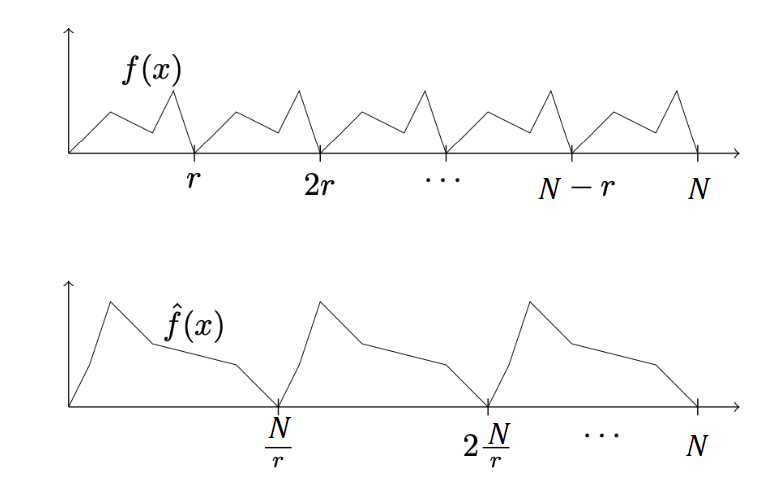
\includegraphics[width=0.8\textwidth]{310/qft_general_case.png}
    \end{center}
}{%
\only<1>{%
\begin{itemize}
    \item The function f(x) repeats every r and its QFT $\hat{f}(x)$ repeats every N/r.
\end{itemize}
}%
}%
%
\textbf{Three variables show the periodic function and QFT:}
\Vskip{-1.5em}\begin{description}
    

    
    \item [$n$] The number of qubits 
    \item [$r$]  The period of the function 
    \item [$N$]  $2^{n}$ The superposition of all possible states the qubits can exist in until they are measured.
   
\end{description}%
    
\end{frame}

\begin{frame}{QFT has period $N/r$ if original function f(x) has period $r$}{Proof Setup: The special f(x) case}
\Vskip{-3em}\TwoColumns{%
\Vskip{-2.5em}\begin{center}
        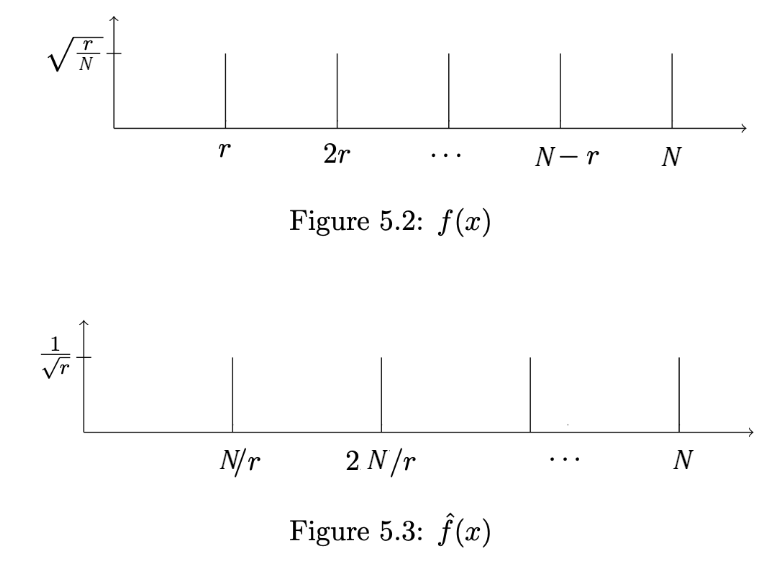
\includegraphics[width=1\textwidth]{310/qft_specific_case.png}
    \end{center}
}{%
\only<1>{%
\begin{itemize}
    \item \[
                f(x) =
                \begin{cases} 
                \sqrt{\frac{r}{N}} & x = 0 \mod{r} \\
                0 & \text{otherwise}
                \end{cases}
            \]
\end{itemize}
}%
}%
%
\Vskip{-1.5em}\begin{itemize}
    \item We will prove our claim for this specific case and use this to extend to the general case. This specific case removes the "noise" anywhere we are not at multiples of the period.

   
\end{itemize}%
    
\end{frame}

\begin{frame}{QFT has period $N/r$ if original function has period $r$}{QFT of special case $f$}
Recall the equation for the QFT
\[ \QFT(\ket{x}) = \RootTwoN{n}\SumPH{y}{n} \ExpPhase{2\pi \frac{y}{2^n} x} \ket{y}\]
Applying this to our function $f(x)$, we get the following equation $\beta_j$ for the $jth$ entry of our QFT $\hat{f}(x)$ (recall $N = {2^n}$, let $\alpha_c$ be the $cth$ entry in our initial state $f(x)$)
\[
\beta_j = \frac{1}{\sqrt{N}} \sum_{c=0}^{N-1} \alpha_c \omega^{cj}
\]
\end{frame}

\begin{frame}{QFT has period $N/r$ if original function has period $r$}{Simplifying $QFT(f) = \hat{f}$}

For our special case function $f(x)$, we can derive the equation for the QFT:
\[
    \hat{f}(x) = \frac{1}{\sqrt{N}} \sum_{j=0}^{\frac{N}{r}-1} \frac{\sqrt{r}}{\sqrt{N}}\omega^{rjx} = \frac{\sqrt{r}}{N} \sum_{j=0}^{\frac{N}{r}-1} \omega^{rjx}
\]

Note that since $f(x) = 0$ at any point that $x \neq 0 \text{(mod r)}$, there will only be $N/r$ nonzero terms that we need to sum. 
% We have also pulled out the constant terms $\frac{1}{\sqrt{N}}$ and $\alpha_j = \frac{\sqrt{r}}{\sqrt{N}}$
\end{frame}

\begin{frame}{QFT has period $N/r$ if original function has period $r$}{Simplifying $QFT(f) = \hat{f}$}
The sum portion can be computed using the equation for the closed form solution to a geometric series.
\[
\sum_{n=0}^{N} a \cdot r^{n} = \frac{a \cdot (r^{N+1} - 1)}{r-1}
\]

Where \(a=1\), \(N=\frac{N}{r}-1\), \(r=\omega^{rx}\), giving:

\[
    \sum_{j=0}^{\frac{N}{r}-1} \omega^{rjx} = \frac{\omega^{Nx}-1}{\omega^{rx}-1}
\]

Since $\omega^{N}$ = 1 (recall $\omega = e^{\frac{2i\pi}{2^n}}$ and $N = 2^n$) our numerator will always be $0$.

Using similar logic, our denominator will be equal to $0$ when $\omega$'s power is equal to $N$ times a constant. We can denote this as $rx = kN$, or $x = \frac{KN}{r} (\mod{\frac{N}{r}})$

\end{frame}

\begin{frame}{QFT has period $N/r$ if original function has period $r$}{Simplifying $QFT(f) = \hat{f}$}
In the case $rx = kN$, or $x = \frac{KN}{r} (\mod{\frac{N}{r}})$ the numerator and denominator will both be 0, so we will use L'Hopital's rule to compute the limit as $x \to \frac{kN}{r}$

\[
   \lim_{x \to \frac{kN}{r}} \frac{\omega^{Nx}-1}{\omega^{rx}-1}
\]

We take the derivative of the top and bottom with respect to $x$ and then simplify using exponent rules.

\[
   \lim_{x \to \frac{kN}{r}} \frac{N}{r} \frac{\omega^{Nx-1}}{\omega^{rx-1}} =  \lim_{x \to \frac{kN}{r}} \frac{N}{r} \frac{\omega^{Nx}\omega^{-1}}{\omega^{rx}\omega^{-1}} = \frac{N}{r}
\]

We are able to simplify to $N/r$ because when we plug in $\frac{kN}{r}$ for $x$ the exponents of $\omega$ are all $N$ times some other constant. Since $\omega^N$ is 1 (recall $\omega = e^{\frac{2\pi i}{N}}$) we can simplify $\omega^{Nx}$ and $\omega^{rx}$ into 1. Then we can simply cancel out terms and are left with $N/r$, which is our period of $QFT(f)$. QED

\end{frame}

\begin{frame}{QFT has period $N/r$ if original function has period $r$}{Example}
We will show in the following example that the function $f(x) = x (mod 2)$ has a period $r = 2$.

We will use a 3-Qubit system so that $N=8$. Generally, it is best to pick $N>>r$. In the first step, we will apply the QFT: 
\[
   \ket{0}\ket{0}\xrightarrow{\text{QFT}_8} \frac{1}{\sqrt{8}}\sum_{x=0}^{7} \ket{x}\ket{0}
\]

Next, we will apply our function:

\[
  \frac{1}{\sqrt{8}}\sum_{x=0}^{7} \ket{x}\ket{0} \xrightarrow{\text{U}_f} \frac{1}{\sqrt{8}}\sum_{x=0}^{7} \ket{x}\ket{x  mod 2}
\]


\end{frame}

\begin{frame}{Measuring the Function Outcome}{Continuation of the Example}
After applying our function, the next step is to measure \( |f\rangle \). Depending on the outcome, \( |f(x)\rangle \) collapses to either \( |0\rangle \) or \( |1\rangle \). For demonstration, assume our measurement returns \( |f(x) = 1\rangle \). This indicates that \( x \) must be odd:

\[
  \frac{1}{\sqrt{8}}\sum_{x=0}^{7} \ket{x} |f(x)\rangle \xrightarrow{\text{measure } |f\rangle} \frac{1}{2}\left( \ket{1} + \ket{3} + \ket{5} + \ket{7} \right) \otimes \ket{1}
\]

Note: Had we measured \( |f\rangle = |0\rangle \) instead, the Fourier transform would only affect the phase, resulting in:

\[
  \frac{1}{2}\left( \ket{0} + \ket{2} + \ket{4} + \ket{6} \right)
\]

\end{frame}

\begin{frame}{Applying the Fourier Transform Again}{Deducing the Period}
To extract the period of the first register without the linear shift, we apply the Fourier transform again:

\[
  \frac{1}{2}\left( \ket{1} + \ket{3} + \ket{5} + \ket{7} \right) \xrightarrow{\text{QFT}_8} \frac{1}{\sqrt{2}} \left( \ket{0} - \ket{4} \right)
\]

With the \( |f\rangle = |0\rangle \) measurement:

\[
  \frac{1}{2}\left( \ket{0} + \ket{2} + \ket{4} + \ket{6} \right) \xrightarrow{\text{QFT}_8} \frac{1}{\sqrt{2}}\left( \ket{0} + \ket{4} \right)
\]

Finally, by taking multiple measurements, one would measure both \( \ket{0} \) and \( \ket{4} \), leading us to deduce \( N/r = 4 \) (since \( N = 8 \)), confirming that \( r = 2 \).

\end{frame}